% Created 2021-06-03 Thu 20:29
% Intended LaTeX compiler: pdflatex

\documentclass[a4paper,12pt]{article}
\usepackage[margin=2cm]{geometry}

\usepackage{hyperref}
\usepackage[utf8]{inputenc}
\usepackage{fixltx2e}
\usepackage{graphicx}
\usepackage{longtable}
\usepackage{float}
\usepackage{wrapfig}
\usepackage{rotating}
\usepackage[normalem]{ulem}
\usepackage{amsmath}
\usepackage{textcomp}
\usepackage{marvosym}
\usepackage{wasysym}
\usepackage{multicol}
\usepackage{amssymb}
\tolerance=1000
\usepackage{listings}
\usepackage{titlesec}
\newcommand{\sectionbreak}{\clearpage}
\usepackage[scaled]{helvet}
\usepackage{courier}
\linespread{1.10}
\usepackage[margin=1.0in]{geometry}
\usepackage[numbers,sort&compress,square]{natbib}
\usepackage{glossaries}
\makeglossaries
\usepackage{setspace} \singlespacing
\usepackage{enumitem}
\setlist[itemize]{noitemsep, topsep=0pt}
\setlist[enumerate]{noitemsep, topsep=0pt}
\setlength\arrayrulewidth{0.7pt} % width of table line
\usepackage[english]{babel}
\addto\captionsenglish{\renewcommand\contentsname{Outline}}
\hypersetup{linktoc = all, colorlinks = true, urlcolor = DodgerBlue4, citecolor = PaleGreen1, linkcolor = black}
\usepackage[UTF8, heading]{ctex}
\usepackage{xltxtra}
\usepackage{xeCJK}
\usepackage{lmodern}
\usepackage{verbatim}
\usepackage{float}
\usepackage{tikz}
\usepackage{wrapfig}
\usepackage{soul}
\usepackage{textcomp}
\usepackage{algorithm}
\usepackage{algorithmic}
\usepackage{marvosym}
\usepackage{wasysym}
\usepackage{natbib}
\usepackage{fancyhdr}
\usepackage{fontspec,xunicode,xltxtra}
\usepackage{CJKnumb}
\usepackage{amsfonts}
\usepackage[default]{sourcecodepro}
\usepackage[T1]{fontenc}
\setCJKmainfont{SimSun} % 設置缺省中文字體
\setmainfont[Scale=0.8]{Times New Roman} % 英文襯線字體
\setsansfont[Scale=0.8]{Source Code Pro} % 英文無襯線字體
\setmonofont[Scale=0.8]{Source Code Pro} % 英文等寬字體
\setCJKmainfont[Scale=0.9]{Adobe Heiti Std} % 中文字體
\setCJKmonofont[Scale=0.9]{Adobe Heiti Std}
\usepackage{color}
\RequirePackage{fancyvrb}
\usepackage{placeins}
\hypersetup{pdfauthor={Name}}
\definecolor{dkgreen}{rgb}{0,0.6,0}
\definecolor{dred}{rgb}{0.545,0,0}
\definecolor{dblue}{rgb}{0,0,0.545}
\definecolor{lgrey}{rgb}{0.9,0.9,0.9}
\definecolor{gray}{rgb}{0.4,0.4,0.4}
\definecolor{darkblue}{rgb}{0.0,0.0,0.6}
\definecolor{bubbles}{rgb}{0.91, 1.0, 1.0}
\definecolor{foreground}{RGB}{220,220,204} % 淺灰
\definecolor{background}{RGB}{62,62,62} % 淺黑
\definecolor{preprocess}{RGB}{250,187,249} % 淺紫
\definecolor{var}{RGB}{239,224,174} % 淺肉色
\definecolor{string}{RGB}{154,150,230} % 淺紫色
\definecolor{type}{RGB}{225,225,116} % 淺黃
\definecolor{function}{RGB}{140,206,211} % 淺天藍
\definecolor{keyword}{RGB}{239,224,174} % 淺肉色
\definecolor{comment}{RGB}{180,98,4} % 深褐色
\definecolor{doc}{RGB}{175,215,175} % 淺鉛綠
\definecolor{comdil}{RGB}{111,128,111} % 深灰
\definecolor{constant}{RGB}{220,162,170} % 粉紅
\lstdefinelanguage{cpp}{ %%定義語言style
backgroundcolor=\color{bubbles},
basicstyle=\footnotesize \ttfamily \color{dblue},
breakatwhitespace=false,
breaklines=true,
captionpos=b,
comment=[l]{\#},
morecomment=[s]{/*}{*/},
commentstyle=\color{comment} \slshape \small \itshape,
ndkeywords={print, printf, repeat, struct, enum, case, switch, func, let, var, boolean, throw, import, typeof, null, catch, switch, for, in, int, str, float, self, return, class, if ,elif, endif, while, do, else, True, False , catch, def},
ndkeywordstyle=\color{dred} \bfseries \small \mono,
identifierstyle=\color{black},
deletekeywords={...},
escapeinside={\%*}{*)},
frame=single,
frameround=tttt,
framesep=0pt,
rulecolor=\color{background},
morekeywords={BRIEFDescriptorConfig,string,TiXmlNode,DetectorDescriptorConfigContainer,istringstream,cerr,exit},
identifierstyle=\color{black},
stringstyle=\color{blue},
rulecolor=\color{black},
showspaces=false,
showstringspaces=false,
showtabs=true,
stepnumber=1,
tabsize=5,
title=\lstname,
}
\lstdefinelanguage{shell}{
backgroundcolor=\color{keyword},
basicstyle=\footnotesize \ttfamily \color{dblue} \small \mono \bfseries,
breakatwhitespace=false,
breaklines=true,
captionpos=b,
comment=[l]{\#},
morecomment=[s]{/*}{*/},
commentstyle=\color{comment} \slshape \small \itshape,
identifierstyle=\color{black},
deletekeywords={...},
escapeinside={\%*}{*)},
frame=single,
frameround=tttt,
framesep=0pt,
rulecolor=\color{background},
morekeywords={BRIEFDescriptorConfig,string,TiXmlNode,DetectorDescriptorConfigContainer,istringstream,cerr,exit},
identifierstyle=\color{black},
stringstyle=\color{blue},
rulecolor=\color{black},
showspaces=false,
showstringspaces=false,
showtabs=false,
stepnumber=1,
tabsize=5,
title=\lstname,
}
\author{Yung Chin, Yen}
\date{\today}
\title{Say Hi to CNN}
\begin{document}

\maketitle
\tableofcontents


\section{神經網路解題步驟}
\label{sec:org82d0fdf}
使用神經網路解決問題可大致分為兩個步驟:「學習」與「推論」。\\
\begin{itemize}
\item 學習指使用訓練資料進行權重參數的學習\\
\item 推論指使用學習過的參數進行資料分類\\
\end{itemize}
而實際的動手實作可再細分為以下幾個步驟\\
\begin{enumerate}
\item 收集資料 (Gathering data)\\
\item 準備數據 (Preparing that data)\\
\item 選擇模型 (Choosing a model)\\
\item 訓練機器 (Training)\\
\item 評估分析 (Evaluation)\\
\item 調整參數 (Hyperparameter tuning)\\
\item 預測推論 (Prediction)\\
\end{enumerate}
\newpage

\section{收集資料}
\label{sec:orgbcd5231}
\subsection{資料類型}
\label{sec:orgb216a64}
\begin{enumerate}
\item 人工收集
\label{sec:org5c6d5ea}
\begin{itemize}
\item 預測股市股價: 開盤、收盤、成交量、技術指標、財務指標、籌碼指標等等\\
\item 以物品識別:大量物品照片並給予名稱(label)\\
\item 以注音符號手寫辨識: 大量手寫照片及其對應答案(label)\\
\end{itemize}
\item 現成資料集
\label{sec:orgc1b8fdf}
\begin{itemize}
\item MNIST\\
資料集由 0\textasciitilde{}9 的數字影像構成(如圖\ref{fig:MNIST-set}),共計 60000 張訓練影像、10000 張測試影像。\\
\begin{figure}[htbp]
\centering
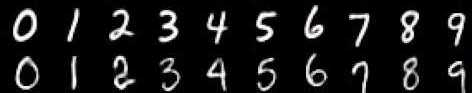
\includegraphics[width=200]{images/MNIST.jpg}
\caption{\label{fig:MNIST-set}MNIST 資料集內容範例}
\end{figure}
\item Boston housing\\
預測目標:房地產價格,特徵包括房地產客觀數據,如年份、平面大小\\
\item Iris\\
鳶尾花資料集是非常著名的生物資訊資料集之一,取自美國加州大學歐文分校的機器學習資料庫,資料的筆數為150筆,共有五個欄位:花萼長度(Sepal Length)、花萼寬度(Sepal Width)、花瓣長度(Petal Length) 、花瓣寬度(Petal Width)、類別(Class):可分為Setosa,Versicolor和Virginica三個品種。\\
\begin{figure}[htbp]
\centering
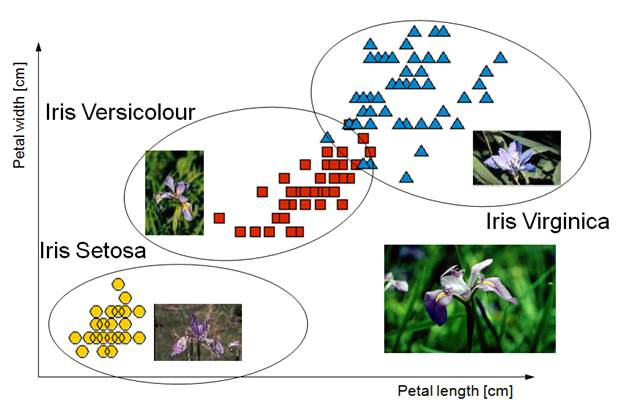
\includegraphics[width=300]{images/cqy409dEexm96zavyuw.png}
\caption{\label{fig:Iris}Iris資料集}
\end{figure}
\item Cifar-10\\
由深度學習大師 Geoffrey Hinton 教授與其在加拿大多倫多大學的學生 Alex Krixhevsky 與 Vinoid Nair 所整理之影像資料集, 包含 6 萬筆 32*32 低解析度之彩色圖片, 其中 5 萬筆為訓練集; 1 萬筆為測試集, 是機器學習中常用的圖片辨識資料集\\
\begin{figure}[htbp]
\centering
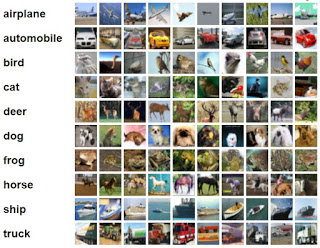
\includegraphics[width=300]{images/cifar10-ten-categories.jpg}
\caption{\label{fig:Cifar10}Cifar-10}
\end{figure}
\end{itemize}
\end{enumerate}

\subsection{DEMO}
\label{sec:orgb72336b}
\lstset{breaklines=true,language=Python,label= ,caption= ,captionpos=b,numbers=none}
\begin{lstlisting}
from keras.datasets import mnist
(x_Train, y_Train), (x_Test, y_Test) = mnist.load_data()
\end{lstlisting}
\newpage

\section{準備數據 (Preparing that data)}
\label{sec:orgefb7a24}
當我們在比較分析兩組數據資料時,可能會遭遇因單位的不同(例如:身高與體重),或數字大小的代表性不同(例如:粉專1萬人與滿足感0.8),造成各自變化的程度不一,進而影響統計分析的結果。\footnote{\href{https://aifreeblog.herokuapp.com/posts/54/data\_science\_203/}{資料的正規化(Normalization)及標準化(Standardization)}\\}\\

資料的正規化(Normalization)是將原始資料的數據按比例縮放於 [0, 1] 區間中,且不改變其原本分佈。\\
\begin{figure}[htbp]
\centering
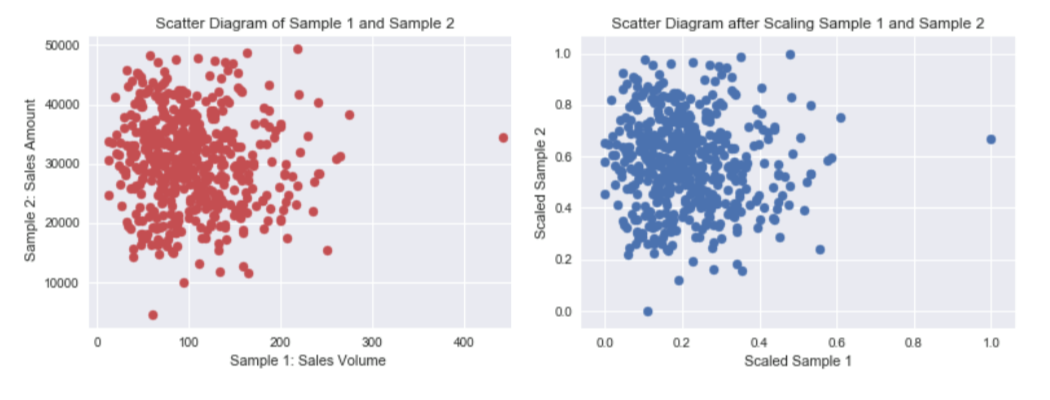
\includegraphics[width=300]{images/normalized.png}
\caption{\label{fig:Name}資料正規化}
\end{figure}

正規化有兩種常用的方法,可以將不同規模的特徵轉化為相同的規模:常態化(normalization)和標準化(standardization):\\
\subsection{常態化}
\label{sec:orgd3576d9}

將特徵值縮化為 0\textasciitilde{}1 間,這是「最小最大縮放」(min-max scaling)的一個特例,某一特徵值的常態化做法如下:\\
$$x_{norm}^i = \frac{x^i-x_{min}}{x_{max}-x_{min}}$$\\
若以 scikit-learn 套件來完成實作,其程式碼如下:\\
\lstset{breaklines=true,language=shell,label= ,caption= ,captionpos=b,numbers=none}
\begin{lstlisting}
from sklearn.preprocessing import MinMaxScaler
mms = MinMaxScaler()
X_train_norm = mms.fit_transform(X_train)
X_test_norm = mms.fit_transform(X_test)
\end{lstlisting}

\subsection{標準化}
\label{sec:org0036f3c}

雖說常態化簡單實用,但對許多機器學習演算法來說(特別是梯度下降法的最佳化),標準化則更為實際,我們可令標準化後的特徵值其平均數為 0、標準差為 1,這樣一來,特徵值會滿足常態分佈,進而使演算法對於離群值不那麼敏感。標準化的公式如下:\\
$$x_{std}^i = \frac{x^i-\mu_x}{\sigma_x}$$\\
若以 scikit-learn 套件來完成實作,其程式碼如下:\\
\lstset{breaklines=true,language=Python,label= ,caption= ,captionpos=b,numbers=none}
\begin{lstlisting}
from sklearn.preprocessing import StandardScaler
stdsc = StandardScaler()
X_train_std = stdsc.fit_transform(X_train)
X_test_std = stdsc.transform(X_test)
\end{lstlisting}

\subsection{DEMO}
\label{sec:org943fe5d}
\lstset{breaklines=true,language=Python,label= ,caption= ,captionpos=b,numbers=none}
\begin{lstlisting}
x_train = x_train.reshape(60000, 784)
x_test = x_test.reshape(10000, 784)
x_train = x_train.astype('float32')
x_test = x_test.astype('float32')
x_train /= 255
x_test /= 255


y_TrainOneHot = np_utils.to_categorical(y_Train)
y_TestOneHot = np_utils.to_categorical(y_Test)
\end{lstlisting}

\section{選擇模型 (Choosing a model)}
\label{sec:orgaea166f}
當數據都進行整理後,接下來就是要選擇訓練用的模型,像是決策樹、LSTM、RNN等等都是機器學習中常使用的訓練模型,其中目前較常拿來訓練股市的是「LSTM」,中文叫做長短期記憶,是屬於深度學習中的一個模型。\\

\subsection{語法}
\label{sec:org1d45e47}
\href{https://keras.io/api/models/model\_training\_apis/}{Keras API reference / Models API / Model training APIs }\\

\subsection{DEMO}
\label{sec:orgd027c45}
\begin{enumerate}
\item LSTM
\label{sec:org51dc121}
\lstset{breaklines=true,language=Python,label= ,caption= ,captionpos=b,numbers=none}
\begin{lstlisting}
model = Sequential()
model.add(LSTM(128,
               input_shape=(x_train.shape[1:]),
               activation='relu',
               return_sequences=True))
model.add(Dropout(0.2))
model.add(LSTM(128, activation='relu'))
model.add(Dropout(0.1))
model.add(Dense(32, activation='relu'))
model.add(Dropout(0.2))
model.add(Dense(10, activation='softmax'))


\end{lstlisting}
\item CNN
\label{sec:orga102c83}
\lstset{breaklines=true,language=Python,label= ,caption= ,captionpos=b,numbers=none}
\begin{lstlisting}
model = Sequential()
model.add(Dense(units=128,
                input_dim=784,
                kernel_initializer='normal',
                activation='relu'))
model.add(Dense(64, activation='relu')
model.add(Dense(units=10,
                kernel_initializer='normal',
                activation='softmax'))


\end{lstlisting}
\begin{figure}[htbp]
\centering
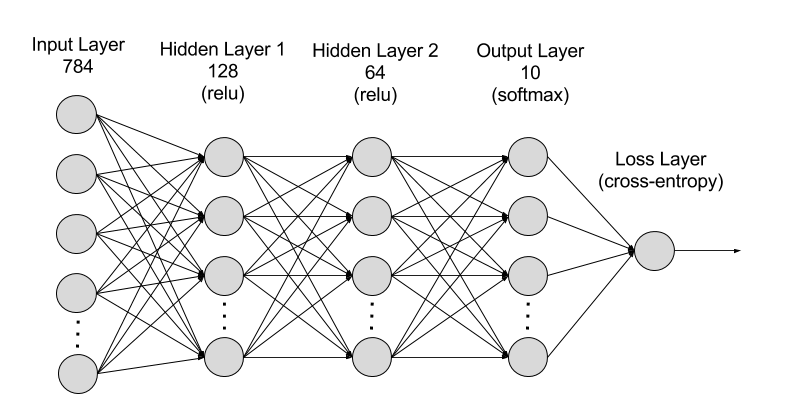
\includegraphics[width=400px]{images/MNIST-CNN.png}
\caption{\label{fig:MNIST-NeuralNet}MNIST-NeuralNet}
\end{figure}
\end{enumerate}

\section{訓練機器 (Training)}
\label{sec:org4774706}

選擇好訓練模型後,再來要將訓練集資料丟進去模型中做訓練,每層要放多少神經元、要跑幾層等等都會影響模型訓練出來的結果,這部分只能靠經驗跟不斷嘗試去學習,或是上網多爬文看別人怎麼撰寫訓練模型\\

在真正訓練前應該再設定好模型的loss function, optimizer。\\
\subsection{語法}
\label{sec:orgd3317ec}
\href{https://keras.io/api/models/model\_training\_apis/}{Keras API reference / Models API / Model training APIs }\\
\subsection{DEMO}
\label{sec:org613ff8a}
\begin{enumerate}
\item LSTM
\label{sec:orge36d9fe}
\lstset{breaklines=true,language=Python,label= ,caption= ,captionpos=b,numbers=none}
\begin{lstlisting}
# ptimizer, loss function
model.compile(optimizer=Adam(lr=0.001),
              loss='categorical_crossentropy',
              metrics=['accuracy'])

model.fit(x_train, y_train,
          epochs=3,
          validation_data=(x_test, y_test))
\end{lstlisting}
\item CNN
\label{sec:org073cf40}
\lstset{breaklines=true,language=Python,label= ,caption= ,captionpos=b,numbers=none}
\begin{lstlisting}
# optimizer, loss function
model.compile(loss='categorical_crossentropy',
              optimizer='adam', metrics=['accuracy'])

model.fit(x=x_Train,
          y=y_TrainOneHot,
          validation_split=0.2,
          epochs=5, batch_size=30, verbose=2)
\end{lstlisting}
\end{enumerate}

\section{評估分析 (Evaluation)}
\label{sec:org3af6549}
當模型訓練完成後,接下來就是判斷該模型是否有過度擬合(overfitting),這裡就是帶入測試集的資料進行評估,也可以嘗試利用交叉驗證的方式進行模型的擬合性判斷,以及利用RESM、MSE等統計計算來判斷模型的準確度\\
\lstset{breaklines=true,language=Python,label= ,caption= ,captionpos=b,numbers=none}
\begin{lstlisting}
scores = model.evaluate(x_Train, y_TestOneHot)
\end{lstlisting}

\section{調整參數 (Hyperparameter tuning)}
\label{sec:org1ee0be2}
到這大致上模型已經完成了50\%,最後的一步就是進行參數的微調,我們也稱為「超參數 (Hyperparamters)」,讓整個模型更加的精準,但也不能過度的調整,因為會造成overfitting的結果,這個取捨就只能依照無窮盡的反覆迭帶去尋找了,這部分也是相對較耗時間的地方\\
\subsection{model參數}
\label{sec:org7de6d2d}
\begin{itemize}
\item 調整model架構: \href{https://medium.com/\%E9\%9B\%9E\%E9\%9B\%9E\%E8\%88\%87\%E5\%85\%94\%E5\%85\%94\%E7\%9A\%84\%E5\%B7\%A5\%E7\%A8\%8B\%E4\%B8\%96\%E7\%95\%8C/\%E6\%A9\%9F\%E5\%99\%A8\%E5\%AD\%B8\%E7\%BF\%92-ml-note-cnn\%E6\%BC\%94\%E5\%8C\%96\%E5\%8F\%B2-alexnet-vgg-inception-resnet-keras-coding-668f74879306}{[機器學習 ML NOTE] CNN演化史(AlexNet、VGG、Inception、ResNet)+Keras Coding}\\
\item loss function: \url{https://keras.io/api/losses/}\\
\item optimizers: \url{https://keras.io/api/optimizers/}\\
\end{itemize}
\subsection{Hyperparameters}
\label{sec:orgc63218d}
\begin{itemize}
\item batch size:一次迭代放入進行訓練或測試的影像數量。\\
\item epoch:一種單位,所有影像皆被計算過1次後即為1 epoch\\
\item \href{http://elmer-storage.blogspot.com/2018/06/cnn-hyperparamters.html}{CNN筆記 - 超參數 (Hyperparamters) }\\
\end{itemize}

\section{預測推論 (Prediction)}
\label{sec:orgb5d60ad}
到此,模型已經正式完成,但對於全新沒影響過的數據則是一個未知數,由於在上方訓練模型中,我們不論是訓練集或是測試集都是被模型所影響過的,如果過度擬合,那麼未來丟入新的資料就很可能無法那麼精準,這部分就只能不斷丟入新資料來推論我們模型的預測能力是否有泛化\\
\lstset{breaklines=true,language=Python,label= ,caption= ,captionpos=b,numbers=none}
\begin{lstlisting}
prediction = model.predict_classes(x_Test4D_normalize)
print(prediction[:10])
\end{lstlisting}

\newpage

\section{DEMO 1: Regression}
\label{sec:orgd162b59}
\subsection{產生數據}
\label{sec:orga951e37}
\lstset{breaklines=true,language=Python,label= ,caption= ,captionpos=b,numbers=none}
\begin{lstlisting}
import matplotlib.pyplot as plt
import numpy as np

x = np.random.uniform(0.0, 3, (2000))
y = 78 + 7.8*x + np.random.normal(0.0, 3, len(x))

plt.scatter(x, y)



x_Train = x[:1500]
x_Test = x[1500:]
y_Train = y[:1500]
y_Test = y[1500:]

\end{lstlisting}

\subsection{建立model}
\label{sec:org0c004fd}
\lstset{breaklines=true,language=Python,label= ,caption= ,captionpos=b,numbers=none}
\begin{lstlisting}
from keras.models import Sequential
from keras.layers import Dense
from keras.layers import Dropout

# A simple regression model
model = Sequential()
model.add(Dense(4, input_shape=(1,)))
model.add(Dropout(0.5))
model.add(Dense(8, input_shape=(1,)))
model.add(Dropout(0.5))
model.add(Dense(1, input_shape=(1,)))
model.compile(loss='mse', optimizer='rmsprop')
\end{lstlisting}

\subsection{訓練model}
\label{sec:org81c7859}
\lstset{breaklines=true,language=Python,label= ,caption= ,captionpos=b,numbers=none}
\begin{lstlisting}
# The fit() method - trains the model
train_history = model.fit(x=x_Train, y=y_Train,
                          validation_split=0.2,
                          epochs=1000, batch_size=200,
                          verbose=0)

\end{lstlisting}

\subsection{查看訓練過程}
\label{sec:orgfdcc124}
\lstset{breaklines=true,language=Python,label= ,caption= ,captionpos=b,numbers=none}
\begin{lstlisting}
print(train_history.history)
print(train_history.history.keys())

import matplotlib.pyplot as plt
plt.title('Train History')
plt.ylabel('loss')
plt.xlabel('Epoch')
plt.plot(train_history.history['loss'])
plt.plot(train_history.history['val_loss'])
plt.show()
\end{lstlisting}

\subsection{評估model}
\label{sec:orgc252e90}
\lstset{breaklines=true,language=Python,label= ,caption= ,captionpos=b,numbers=none}
\begin{lstlisting}
# The evaluate() method - gets the loss statistics
score = model.evaluate(x_Test, y_Test, batch_size=200)
print(score)
\end{lstlisting}

\subsection{預測結果}
\label{sec:org05e0d85}
\lstset{breaklines=true,language=Python,label= ,caption= ,captionpos=b,numbers=none}
\begin{lstlisting}
# The predict() method - predict the outputs for the given inputs
model.predict(np.expand_dims(x_Test[:3],1))
print(x_Test[:3])
print(y_Test[:3])
model.predict(x_Test[:3])
\end{lstlisting}

\subsection{調整model/參數}
\label{sec:org74753e2}
\begin{enumerate}
\item model架構
\label{sec:org8ebde86}
\item loss function
\label{sec:org73d2a71}
\item optimizer
\label{sec:org38b55fc}
\item hyper parameters
\label{sec:org1a20d2b}
\item \#1
\label{sec:org7fcdcb5}
\lstset{breaklines=true,language=Python,label= ,caption= ,captionpos=b,numbers=none}
\begin{lstlisting}
# A simple regression model
model = Sequential()
model.add(Dense(4, input_shape=(1,)))
model.add(Dense(8, input_shape=(1,)))
model.add(Dense(4, input_shape=(1,)))
model.add(Dense(1, input_shape=(1,)))
model.compile(loss='mean_squared_error', optimizer='rmsprop')
#mean_squared_logarithmic_error
#mean_absolute_percentage_error

\end{lstlisting}

\item \#2
\label{sec:org7266519}
\lstset{breaklines=true,language=Python,label= ,caption= ,captionpos=b,numbers=none}
\begin{lstlisting}
model = Sequential()
model.add(Dense(4, input_shape=(1,)))
model.add(Dense(8, input_shape=(1,)))
model.add(Dense(16, input_shape=(1,)))
model.add(Dense(32, input_shape=(1,)))
model.add(Dense(16, input_shape=(1,)))
model.add(Dense(4, input_shape=(1,)))
model.add(Dense(1, input_shape=(1,)))
model.compile(loss='mse', optimizer='rmsprop') 
\end{lstlisting}
\end{enumerate}

\section{練習: Regression}
\label{sec:orgbd184da}
\subsection{數據}
\label{sec:org26a3c23}
\lstset{breaklines=true,language=Python,label= ,caption= ,captionpos=b,numbers=none}
\begin{lstlisting}
import numpy as np

# Seed the random number generator for reproducibility
np.random.seed(0)

x_data = np.linspace(-10, 10, num=2000)
y_data = 2.9 * np.sin(1.5 * x_data) + np.random.normal(size=len(x_data))

plt.scatter(x_data, y_data)
\end{lstlisting}

\begin{figure}[htbp]
\centering
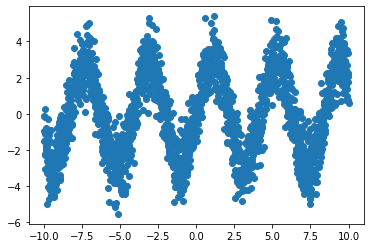
\includegraphics[width=300]{images/random_curve.png}
\caption{\label{fig:CNN_practice}CNN練習}
\end{figure}
\newpage

\section{DEMO 2: MNIST 資料集}
\label{sec:org9e0f173}
\subsection{MNIST}
\label{sec:orgc481e60}
\begin{itemize}
\item MNIST 是機器學習領域中相當著名的資料集,號稱機器學習領域的「Hello world.」,其重要性不言可喻。\\
\item MNIST 資料集由 0\textasciitilde{}9 的數字影像構成(如圖\ref{fig:MNIST-set}),共計 60000 張訓練影像、10000 張測試影像。\\
\item 一般的 MMIST 資料集的用法為:使用訓練影像進行學習,再利用學習後的模型預測能否正確分類測試影像。\\
\end{itemize}

準備資料是訓練模型的第一步,基礎資料可以是網上公開的資料集,也可以是自己的資料集。視覺、語音、語言等各種型別的資料在網上都能找到相應的資料集。\\

\subsection{準備 MNIST 資料}
\label{sec:org6c76893}
MNIST 數據集來自美國國家標準與技術研究所, National Institute of Standards and Technology (NIST). 訓練集 (training set) 由來自 250 個不同人手寫的數字構成, 其中 50\% 是高中學生, 50\% 來自人口普查局 (the Census Bureau) 的工作人員. 測試集(test set) 也是同樣比例的手寫數字數據。MNIST 數據集可在 \url{http://yann.lecun.com/exdb/mnist/} 獲取, 它包含了四個部分:\\
\begin{enumerate}
\item Training set images: train-images-idx3-ubyte.gz (9.9 MB, 解壓後 47 MB, 包含 60,000 個樣本)\\
\item Training set labels: train-labels-idx1-ubyte.gz (29 KB, 解壓後 60 KB, 包含 60,000 個標籤)\\
\item Test set images: t10k-images-idx3-ubyte.gz (1.6 MB, 解壓後 7.8 MB, 包含 10,000 個樣本)\\
\item Test set labels: t10k-labels-idx1-ubyte.gz (5KB, 解壓後 10 KB, 包含 10,000 個標籤)\\
\end{enumerate}

\begin{enumerate}
\item load data
\label{sec:orge5dc1a1}
MNIST 資料集是一個適合拿來當作 TensotFlow 的練習素材,在 Tensorflow 的現有套件中,也已經有內建好的 MNIST 資料集,我們只要在安裝好 TensorFlow 的 Python 環境中執行以下程式碼,即可將 MNIST 資料成功讀取進來。.\\
\lstset{breaklines=true,language=Python,label= ,caption= ,captionpos=b,numbers=none}
\begin{lstlisting}
import tensorflow as tf
mnist = tf.keras.datasets.mnist
(x_train, y_train), (x_test, y_test) = mnist.load_data()      (get-keras-mnist)
\end{lstlisting}
在訓練模型之前,需要將樣本資料劃分為訓練集、測試集,有些情況下還會劃分為訓練集、測試集、驗證集。由上述程式第get-keras-mnist行可知,下載後的 MNIST 資料分成訓練資料(training data)與測試資料(testing data),其中 x 為圖片、y為所對應數字。\\
\lstset{breaklines=true,language=Python,label= ,caption= ,captionpos=b,numbers=none}
\begin{lstlisting}
import tensorflow as tf
mnist = tf.keras.datasets.mnist
(x_train, y_train), (x_test, y_test) = mnist.load_data()
# =====================================
# 判斷資料形狀
print(x_train.shape)
print(x_test.shape)
# 第一個label的內容
print(y_train[0])
# 顯示影像內容
import matplotlib.pylab as plt
img = x_train[0]
plt.imshow(img)
plt.savefig("MNIST-Image.png")
\end{lstlisting}
由上述程式輸出結果可以看到載入的 x 為大小為 28*28 的圖片共 60000 張,每一筆 MNIST 資料的照片(x)由 784 個 pixels 組成(28*28),照片內容如圖\ref{fig:MNIST-Image},訓練集的標籤(y)則為其對應的數字(0~9),此例為 5。\\
\begin{figure}[htbp]
\centering
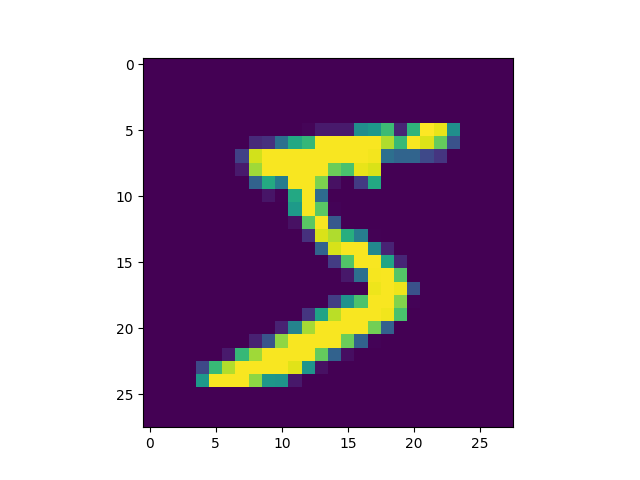
\includegraphics[width=100px]{images/MNIST-Image.png}
\caption{\label{fig:MNIST-Image}MNIST 影像示例}
\end{figure}

x 的影像資料為灰階影像,每個像素的數值介於 0\textasciitilde{}255 之間,矩陣裡每一項的資料則是代表每個 pixel 顏色深淺的數值,如下圖\ref{fig:MNIST-Matrix}所示:\\
\begin{figure}[htbp]
\centering
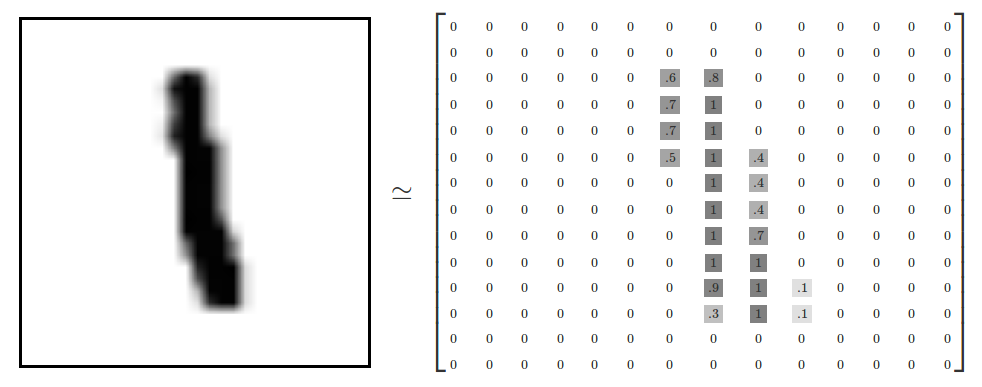
\includegraphics[width=200]{images/MNIST-Matrix.png}
\caption{\label{fig:MNIST-Matrix}MNIST 資料矩陣}
\end{figure}

載入的 y 為所對應的數字 0\textasciitilde{}9,在這我們要運用 keras 中的 np\_under\_utils.to\_under\_categorical 將 y 轉成 one-hot 的形式,將他轉為一個 10 維的 vector,例如:我們所拿到的資料為 y=3,經過 np\_utils.to\_categorical,會轉換為 y=[0,0,0,1,0,0,0,0,0,0]。這部份的轉換程式碼如下:\\
\lstset{breaklines=true,language=Python,label= ,caption= ,captionpos=b,numbers=none}
\begin{lstlisting}
from keras.datasets import mnist
from keras.utils import np_utils
import tensorflow as tf

mnist = tf.keras.datasets.mnist
(x_train, y_train), (x_test, y_test) = mnist.load_data()
# =====================================
# 將圖片轉換為一個60000*784的向量,並且標準化
x_train = x_train.reshape(60000, 784).astype('float32')
x_test = x_test.reshape(10000, 784).astype('float32')
x_train = x_train/255
x_test = x_test/255
# 將y轉換成one-hot encoding
y_train = np_utils.to_categorical(y_train, 10)
y_test = np_utils.to_categorical(y_test, 10)
# 回傳處理完的資料
print(y_train[0])

import numpy as np
np.set_printoptions(precision=2)
#print(x_train[0])
\end{lstlisting}
\end{enumerate}

\subsection{MNIST 的推論處理}
\label{sec:org3f28b51}

如圖\ref{fig:MNIST-NeuralNet}所示,MNIST 的推論神經網路最前端的輸入層有 784 (\(28*28=784\))個神經元,最後的輸出端有 10 個神經元(\(0~9\)個數字),至於中間的隠藏層有兩個,第 1 個隱藏層有 50 個神經元,第 2 層有 100 個。此處的 50、100 可以設定為任意數(如,也可以是 128、64)。\\
\begin{figure}[htbp]
\centering
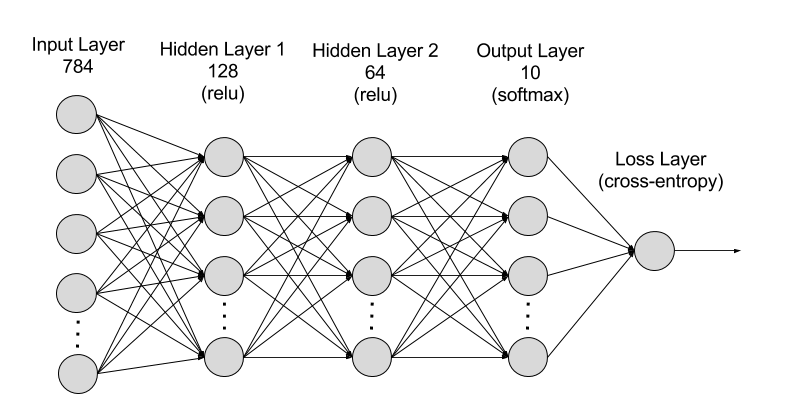
\includegraphics[width=400px]{images/MNIST-CNN.png}
\caption{\label{fig:MNIST-NeuralNet}MNIST-NeuralNet}
\end{figure}

\subsection{MNIST 資料集:以 DNN Sequential 模型為例}
\label{sec:org6aba738}

此處以最簡單的 DNN (deep neural network) 作為範例。以 Keras 的核心為模型,應用最常使用 Sequential 模型。藉由.add()我們可以一層一層的將神經網路疊起。在每一層之中我們只需要簡單的設定每層的大小(units)與激活函數(activation function)。需要特別記得的是:第一層要記得寫輸入的向量大小、最後一層的 units 要等於輸出的向量大小。在這邊我們最後一層使用的激活函數(activation function)為 softmax。\\

\begin{enumerate}
\item Import Library
\label{sec:orgb0ccc13}
\lstset{breaklines=true,language=Python,label= ,caption= ,captionpos=b,numbers=none}
\begin{lstlisting}
from keras.datasets import mnist
from keras.utils import np_utils
import numpy as np
np.random.seed(10)
\end{lstlisting}

\item 資料預處理
\label{sec:orgde9b677}
\lstset{breaklines=true,language=Python,label= ,caption= ,captionpos=b,numbers=none}
\begin{lstlisting}
(x_Train, y_Train), (x_Test, y_Test) = mnist.load_data()
import matplotlib.pyplot as plt

##print(x_Train[1].shape)
#print(x_Train[1])
#plt.imshow(x_Train[1])
##y_Train[1]

x_Train=x_Train.reshape(x_Train.shape[0],28,28,1).astype('float32')
x_Test=x_Test.reshape(x_Test.shape[0],28,28,1).astype('float32')
#x_Train4D[1].shape
#print(x_Train4D[1])

x_Train = x_Train / 255
x_Test = x_Test / 255

y_Train = np_utils.to_categorical(y_Train)
y_Test = np_utils.to_categorical(y_Test)
\end{lstlisting}

\item 建立模型
\label{sec:org4f33506}
\lstset{breaklines=true,language=Python,label= ,caption= ,captionpos=b,numbers=none}
\begin{lstlisting}
model = Sequential()
#將模型疊起
model.add(Dense(input_dim=28*28,units=128,activation='relu'))
model.add(Dense(units=64,activation='relu'))
model.add(Dense(units=10,activation='softmax'))
# model.summary()
\end{lstlisting}

\item 訓練模型
\label{sec:org45e5efd}
\lstset{breaklines=true,language=Python,label= ,caption= ,captionpos=b,numbers=none}
\begin{lstlisting}
model.compile(loss='categorical_crossentropy',
              optimizer='adam',metrics=['accuracy'])

train_history=model.fit(x=x_Train,
                        y=y_Train,validation_split=0.2,
                        epochs=6, batch_size=300,verbose=2)
\end{lstlisting}

\item 查看訓練過程
\label{sec:orgb6feed2}
\lstset{breaklines=true,language=Python,label= ,caption= ,captionpos=b,numbers=none}
\begin{lstlisting}
import matplotlib.pyplot as plt
def show_train_history(train_acc,test_acc):
    plt.plot(train_history.history[train_acc])
    plt.plot(train_history.history[test_acc])
    plt.title('Train History')
    plt.ylabel('Accuracy')
    plt.xlabel('Epoch')
    plt.legend(['train', 'test'], loc='upper left')
    plt.show()

show_train_history('accuracy','val_accuracy')
show_train_history('loss','val_loss')
\end{lstlisting}

\item 評估模型準確率
\label{sec:org1541fec}
\lstset{breaklines=true,language=Python,label= ,caption= ,captionpos=b,numbers=none}
\begin{lstlisting}
scores = model.evaluate(x_Test , y_Test, batch_size = 200)
scores[1]
\end{lstlisting}

\item 實際預測結果
\label{sec:org26cf554}
\lstset{breaklines=true,language=Python,label= ,caption= ,captionpos=b,numbers=none}
\begin{lstlisting}
prediction=model.predict_classes(x_Test)
prediction[:10]

import matplotlib.pyplot as plt
def plot_images_labels_prediction(images,labels,prediction,idx,num=10):
    fig = plt.gcf()
    fig.set_size_inches(12, 14)
    if num>25: num=25
    for i in range(0, num):
        ax=plt.subplot(5,5, 1+i)
        ax.imshow(images[idx], cmap='binary')

        ax.set_title("label=" +str(labels[idx])+
                     ",predict="+str(prediction[idx])
                     ,fontsize=10)

        ax.set_xticks([]);ax.set_yticks([])
        idx+=1
    plt.show()
plot_images_labels_prediction(x_Test,y_Test,prediction,idx=0) #要用到原始的值
\end{lstlisting}

\item confusion matrix
\label{sec:org355b86a}
\lstset{breaklines=true,language=Python,label= ,caption= ,captionpos=b,numbers=none}
\begin{lstlisting}
import pandas as pd
pd.crosstab(y_Test,prediction,
            rownames=['label'],colnames=['predict'])
\end{lstlisting}

\lstset{breaklines=true,language=Python,label= ,caption= ,captionpos=b,numbers=none}
\begin{lstlisting}
# 載入資料
from keras.datasets import mnist
from keras.utils import np_utils

def load_data():
    # 載入minst的資料
    (x_train, y_train), (x_test, y_test) = mnist.load_data()
    # 將圖片轉換為一個60000*784的向量,並且標準化
    x_train = x_train.reshape(x_train.shape[0], 28*28)
    x_test = x_test.reshape(x_test.shape[0], 28*28)
    x_train = x_train.astype('float32')
    x_test = x_test.astype('float32')
    x_train = x_train/255
    x_test = x_test/255
    # 將y轉換成one-hot encoding
    y_train = np_utils.to_categorical(y_train, 10)
    y_test = np_utils.to_categorical(y_test, 10)
    # 回傳處理完的資料
    return (x_train, y_train), (x_test, y_test)

import numpy as np
from keras.models import Sequential
from keras.layers.core import Dense,Activation
from keras.optimizers import  Adam

def build_model():#建立模型
    model = Sequential()
    #將模型疊起
    model.add(Dense(input_dim=28*28,units=128,activation='relu'))
    model.add(Dense(units=64,activation='relu'))
    model.add(Dense(units=10,activation='softmax'))
    model.summary()
    return model

# 開始訓練模型,此處使用了Adam做為我們的優化器,loss function選用了categorical_crossentropy。
(x_train,y_train),(x_test,y_test)=load_data()
model = build_model()
#開始訓練模型
model.compile(loss='categorical_crossentropy',optimizer="adam",metrics=['accuracy'])
model.fit(x_train,y_train,batch_size=100,epochs=5)
#顯示訓練結果
score = model.evaluate(x_train,y_train)
print ('\nTrain Acc:', score[1])
score = model.evaluate(x_test,y_test)
print ('\nTest Acc:', score[1])

### 進行預測
prediction = model.predict_classes(x_Test4D_normalize)
print(prediction[:10])
plot_images_labels_prediction("CNN_MNist", x_Test, y_Test, prediction, idx=0)
import pandas as pd
p = pd.crosstab(y_Test, prediction, rownames=['label'], colnames=['predict'])
print(p)

\end{lstlisting}

\begin{verbatim}
_________________________________________________________________
Layer (type)                 Output Shape              Param #
=================================================================
dense_1 (Dense)              (None, 500)               392500
_________________________________________________________________
dense_2 (Dense)              (None, 500)               250500
_________________________________________________________________
dense_3 (Dense)              (None, 500)               250500
_________________________________________________________________
dense_4 (Dense)              (None, 10)                5010
=================================================================
Total params: 898,510
Trainable params: 898,510
Non-trainable params: 0
_________________________________________________________________
Epoch 1/20

  100/60000 [..............................] - ETA: 2:55 - loss: 2.2917 - acc: 0.1300
  800/60000 [..............................] - ETA: 25s - loss: 1.6424 - ACM: 0.5362
.......
16300/60000 [=======>......................] - ETA: 4s - loss: 0.3752 - acc: 0.8898
17000/60000 [=======>......................] - ETA: 4s - loss: 0.3681 - acc: 0.8916
.......
50600/60000 [========================>.....] - ETA: 0s - loss: 0.2232 - acc: 0.9335
51300/60000 [========================>.....] - ETA: 0s - loss: 0.2220 - acc: 0.9338
.......
59700/60000 [============================>.] - ETA: 0s - loss: 0.2078 - acc: 0.9377
60000/60000 [==============================] - 5s 81us/step - loss: 0.2074 - acc: 0.9379
Epoch 2/20

  100/60000 [..............................] - ETA: 5s - loss: 0.0702 - acc: 0.9800
......
60000/60000 [==============================] - 5s 77us/step - loss: 0.0832 - acc: 0.9740
Epoch 3/20
......
Epoch 29/20

   32/60000 [..............................] - ETA: 1:10
 1440/60000 [..............................] - ETA: 3s
......
58496/60000 [============================>.] - ETA: 0s
60000/60000 [==============================] - 2s 34us/step

Train Acc: 0.9981666666666666

   32/10000 [..............................] - ETA: 0s
 1568/10000 [===>..........................] - ETA: 0s
 3104/10000 [========>.....................] - ETA: 0s
 4640/10000 [============>.................] - ETA: 0s
 6176/10000 [=================>............] - ETA: 0s
 7680/10000 [======================>.......] - ETA: 0s
 9184/10000 [==========================>...] - ETA: 0s
10000/10000 [==============================] - 0s 33us/step

Test Acc: 0.9823
\end{verbatim}


\newpage
\end{enumerate}

\section{作業二}
\label{sec:org9456fba}
\subsection{背景}
\label{sec:orgee4de4a}
某醫學研究中心針對旗下醫院800名疑似患有「無定向喪心病狂間歇性全身機能失調症」的患者做了一份病徵研究,針對以下這些可能病徵進行程度檢驗\\
\begin{enumerate}
\item 抑鬱\\
\item 癲癇\\
\item 精神分裂\\
\item 輕挑驕傲\\
\item 沒大沒小\\
\item 有犯罪傾向\\
\item 月經前緊張(男患者嚴重的話也有)\\
\item 有自殺傾向\\
\end{enumerate}
這800份資料可以\href{https://letranger.github.io/downloads/qq.csv}{點選這裡}下載,每筆資料有九個欄位,前八欄分別對應到上述八項病徵,最後一欄為0/1,代表病患是否患有該病。\\

請你建立一個預測MODEL,以利該中心將來遇到類似病情的患者時只要先針對這些特徵值進行檢驗,即可了解該病例是否為此病患者,並即時予以適當治療。\\
\subsection{作業要求}
\label{sec:org492d5bc}
\end{document}
